\documentclass[a4paper,11pt]{article}
\usepackage[utf8]{inputenc}
\usepackage[frenchb]{babel}
\usepackage{amssymb}
\usepackage{amsmath}
\usepackage{amsthm}
\usepackage{mathrsfs}
\usepackage{array}
\usepackage{graphicx}
\usepackage[usenames,dvipsnames]{color}
\usepackage{listings}
\usepackage{arydshln}
\usepackage{multirow}
%\usepackage{slashbox}
\usepackage{subfigure}
\usepackage{pdflscape}
%\usepackage{cancel}
%\usepackage[bookmarks = false]{hyperref}
\usepackage[left=1.75cm, right=1.75cm, top=2cm, bottom=2cm]{geometry}

\newcommand{\ttsee}[1]{Voir \texttt{#1}\paragraph{}}
\newcommand{\ttseek}[1]{Voir package \texttt{#1}\paragraph{}}


% Initialisation de listings
%\definecolor{mymauve}{rgb}{0.63,0.13,0.94}
%\definecolor{mygreen}{rgb}{0.13,0.55,0.13}
%\definecolor{mybeige}{rgb}{0.99,0.99,0.86}
%\definecolor{mygris}{rgb}{0.8,0.8,0.8}
\definecolor{light-gray}{gray}{0.50}
\lstset{
    columns=flexible,
	%numbers = left,				% placement de la numérotation des lignes
	numberstyle = \small,        	% taille du numéro de ligne
	stepnumber = 1,              	% ???
	numbersep = 10pt,            	% taille de l'espace de séparation entre numéro de ligne et code
	showspaces = false,          	% montrer les espaces
	showstringspaces=false,         % enlever les espaces str
	showtabs = false,            	% montrer les tabulations
	tab = rightarrowfill,        	% ???
	tabsize=3,						% tabulation size
	language = Java,             	% langage utilisé
	basicstyle = \footnotesize\tt,	% ???
	captionpos = b,					% ???
	linewidth=\linewidth,			% largeur de la fenetre de code
	breaklines = true,				% ???
	commentstyle = \color{light-gray}, % définition de la couleur des commentaires
	%stringstyle = \color{mymauve},  % définition de la couleur des chaines de caractères
	%identifierstyle = \ttfamily,    % ???
	keywordstyle = \color{blue},	% définition de la couleur des mots clés
	%frame=single,
	%backgroundcolor=\color{mybeige},
	extendedchars=true				% étend les caractères pouvant être utilisés
}

%\author{Mormont Romain}
%\title{Synthèse : Base de données (Pierre Wolper)}
%\date{Année académique 2013-2014}

\begin{document}
\rule{1\linewidth}{1px}
{ \sc
\begin{center}
{\small University of Liège}\\
{\small Faculty of Applied Sciences}

\end{center}

\vfill
\begin{center}

{\Huge Object Oriented Software Engineering {\LARGE \tt [INFO0063]}\\}
\end{center}
\begin{center}
{\Huge Project : Report}
\end{center}
\begin{center}
\textbf{Magera Floriane}\\
{\small 1$^{\text{st}}$ master in computer engineering}\\
{\small Option : Computer systems and networks}\\
{\small s111295}\\
\vspace{0.5cm}
\textbf{Servais Fabrice}\\
{\small 1$^{\text{st}}$ master in computer engineering}\\
{\small Option : Computer systems and networks}\\
{\small s111093}\\
\vspace{0.5cm}
\textbf{Mormont Romain}\\
{\small 1$^{\text{st}}$ master in computer engineering}\\
{\small Option : Intelligent systems}\\
{\small s110940}
\end{center}

\vfill
\begin{center}
Academic year 2014-2015\\
\end{center}
}
\rule{1\linewidth}{1px}
\newpage
\tableofcontents
\newpage

\section{Introduction}

This report presents the solution we have developed for the INFO0063 course project. In the Section \ref{sec:diagrams}, we will first discuss about the diagrams we have chosen for describing the concept and design of the application. In the Section \ref{sec:patterns}, we will present the patterns we have included in our solution and, finally, in the Section \ref{sec:cls_hier}, we will say few words about our class hierarchy.

\section{Diagrams}
\label{sec:diagrams}
	
	\subsection{Conceptual}

At the conceptual level, we provide 2 diagrams of different kinds to show the whole program : class and activity diagrams.

\paragraph{}





\subsection{Design}
We have chosen sequence and class diagrams to document our application design. 
\subsubsection{Interfaces}
The interfaces are given in the diagram in Figure \ref{fig:inter}.
\subsubsection{Logic}
The logic core class is the \texttt{Logic} class which implements the logic interface and is thus the main entry point of the logic subsystem. The others entry-points are the cells. This class interacts with the following :
\begin{itemize}
	\item reversible actions : classes \texttt{Stack<Command>}, \texttt{Command} and \texttt{Rotation} 
	\item game board : classes \texttt{Board} and \texttt{Cell}
	\item configuration file parsing : class \texttt{Parser}
	\item chronometer : class \texttt{PeriodicNotifier}
\end{itemize}
These components are described in the diagram in Figure.
\subsubsection{Cells}
As board cell
\subsubsection{Algorithms and data structures}
\section{Applied patterns}
\subsection{Observer}
\subsection{Command}
\subsection{Builder and singleton}
\label{sec:patterns}
\section{Class hierarchy}
\label{sec:cls_hier}
\section{Conclusion}
\appendix
\section{Conceptual}
\subsection{Class diagrams}
\begin{figure}[h]
	\center
	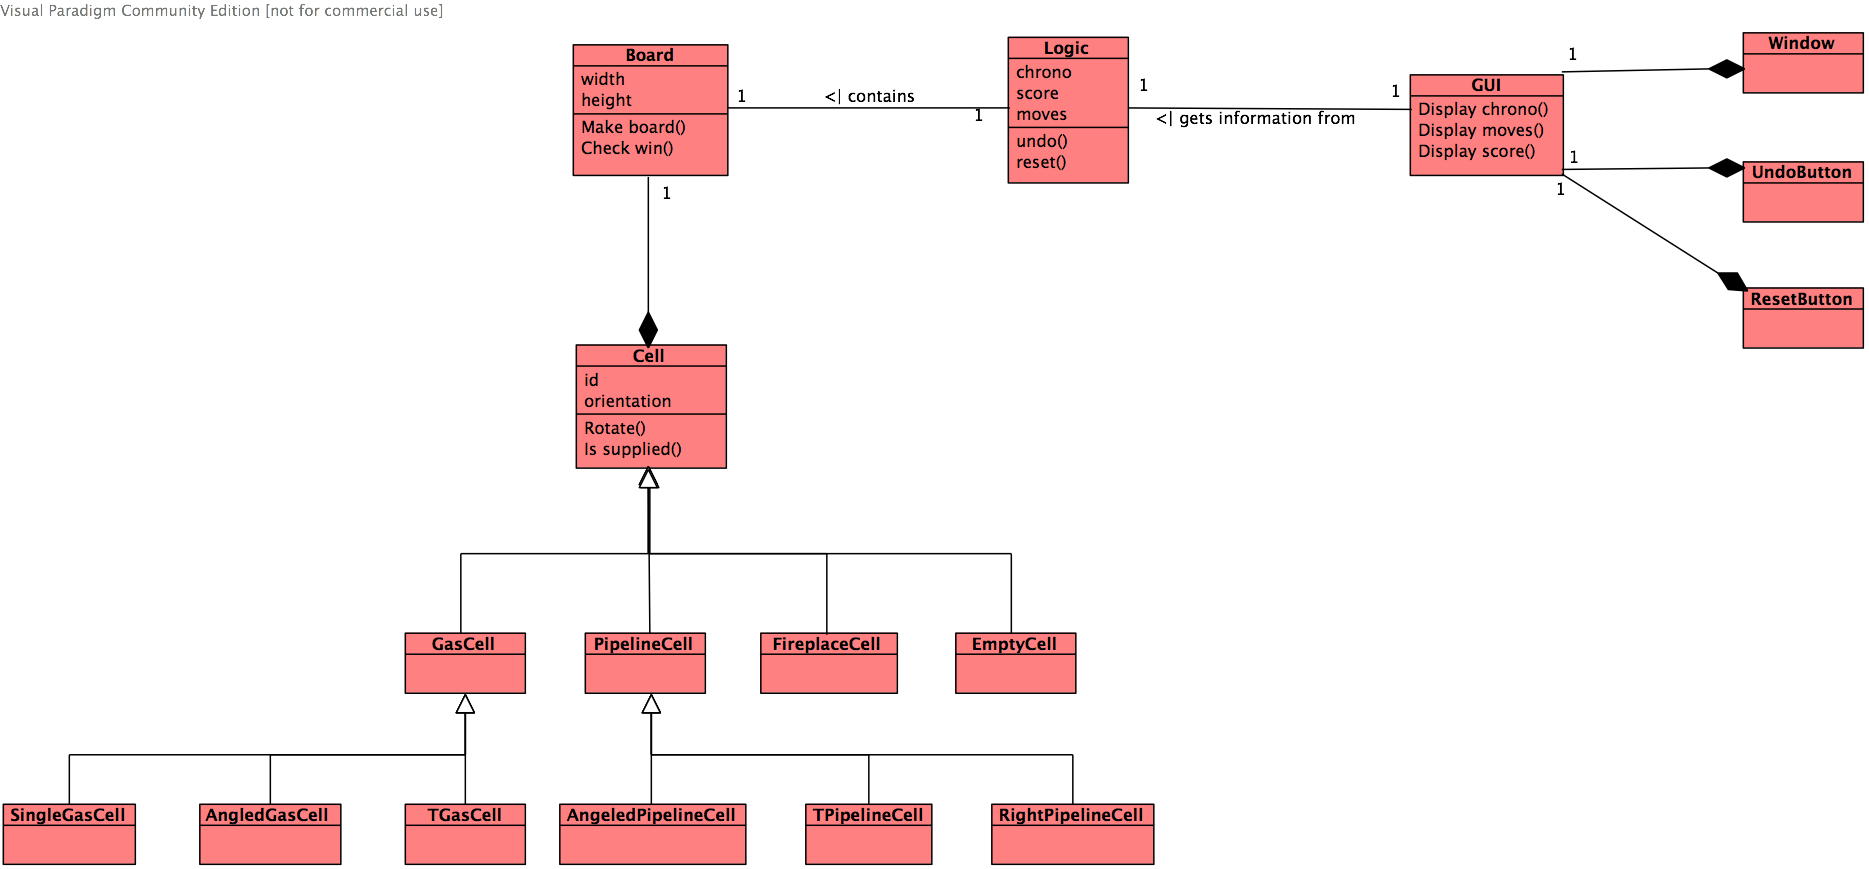
\includegraphics[angle=90,scale=0.8]{Conceptual-Class-diagram.png}
	\caption{Conceptual class diagram}
	\label{fig:concept-class}
\end{figure}

\subsection{Activity diagram}
\begin{figure}[h]
	\center
	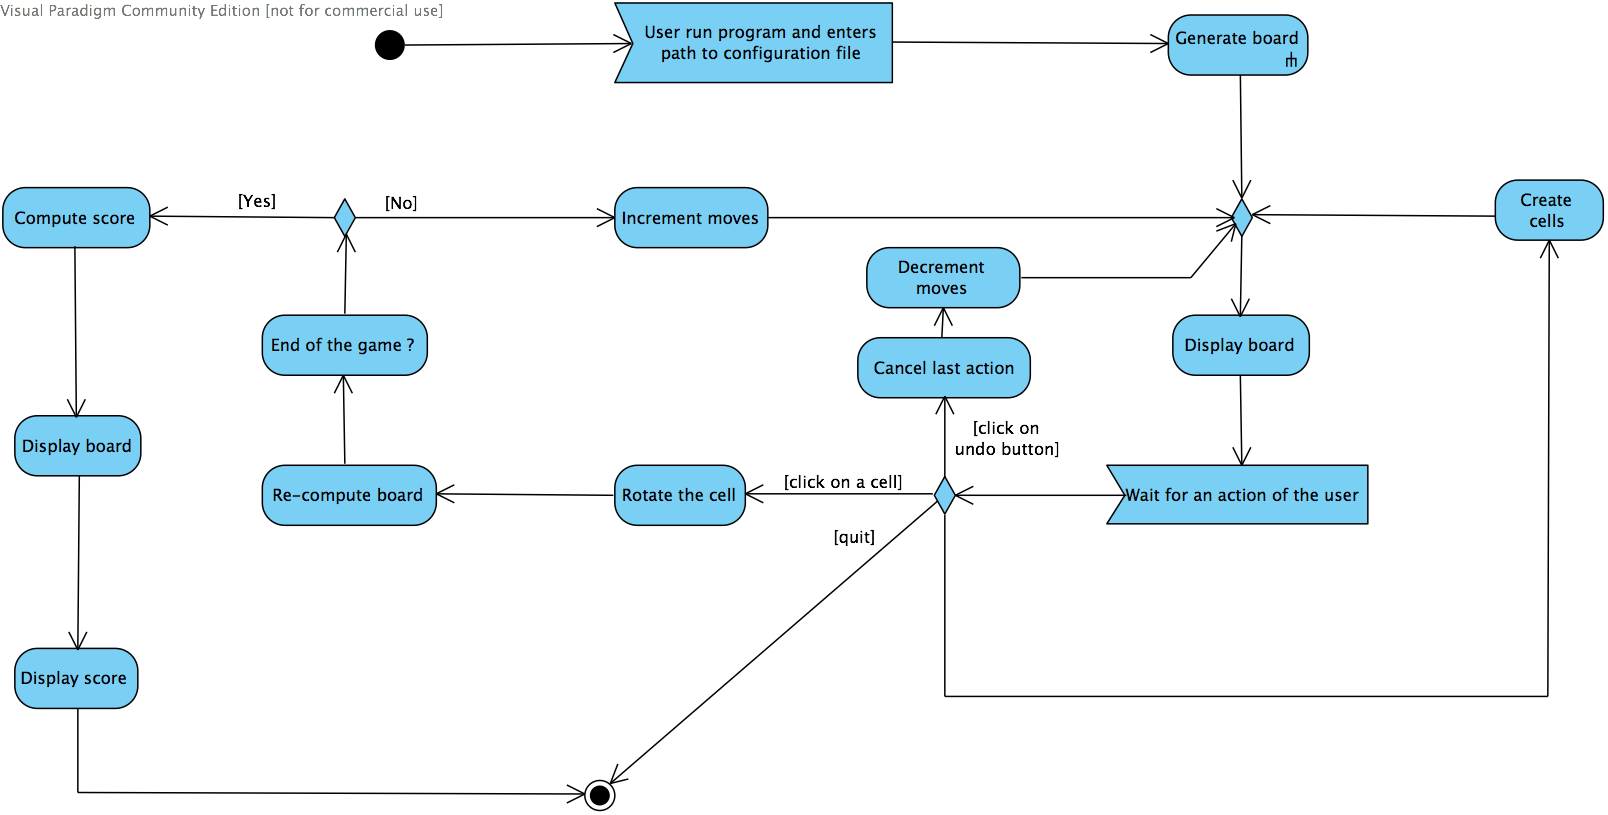
\includegraphics[angle=90,scale=0.9]{Conceptual-activity-diagram.png}
	\caption{Conceptual activity diagram - Game}
	\label{fig:concept-activity}
\end{figure}

\begin{figure}[h]
	\center
	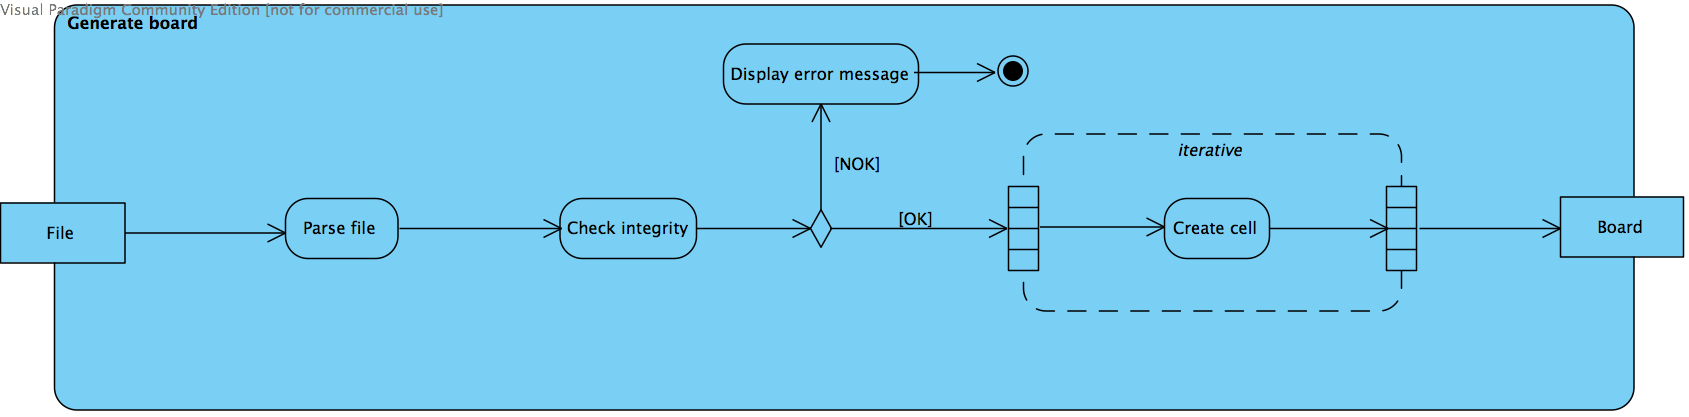
\includegraphics[angle=90,scale=0.7]{Generate-board.png}
	\caption{Conceptual sub-activity diagram - Generate board}
	\label{fig:concept-generate-board}
\end{figure}

\section{Design}
\subsection{Class diagrams}
\begin{figure}[h]
	\center
	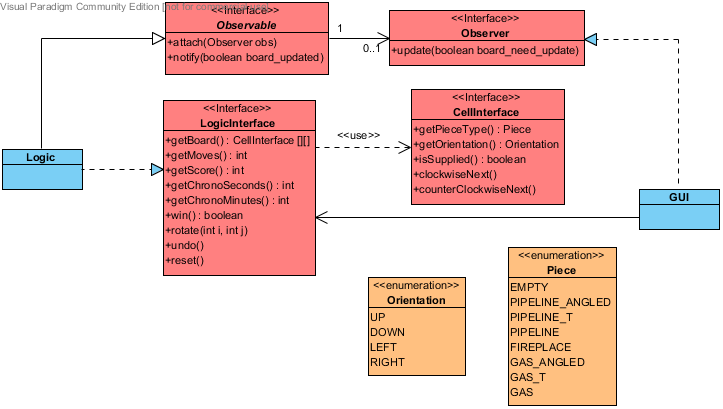
\includegraphics[angle=90,scale=1]{interfaces.png}
	\caption{Interfaces}
	\label{fig:inter}
\end{figure}
\begin{figure}[h]
	\center
	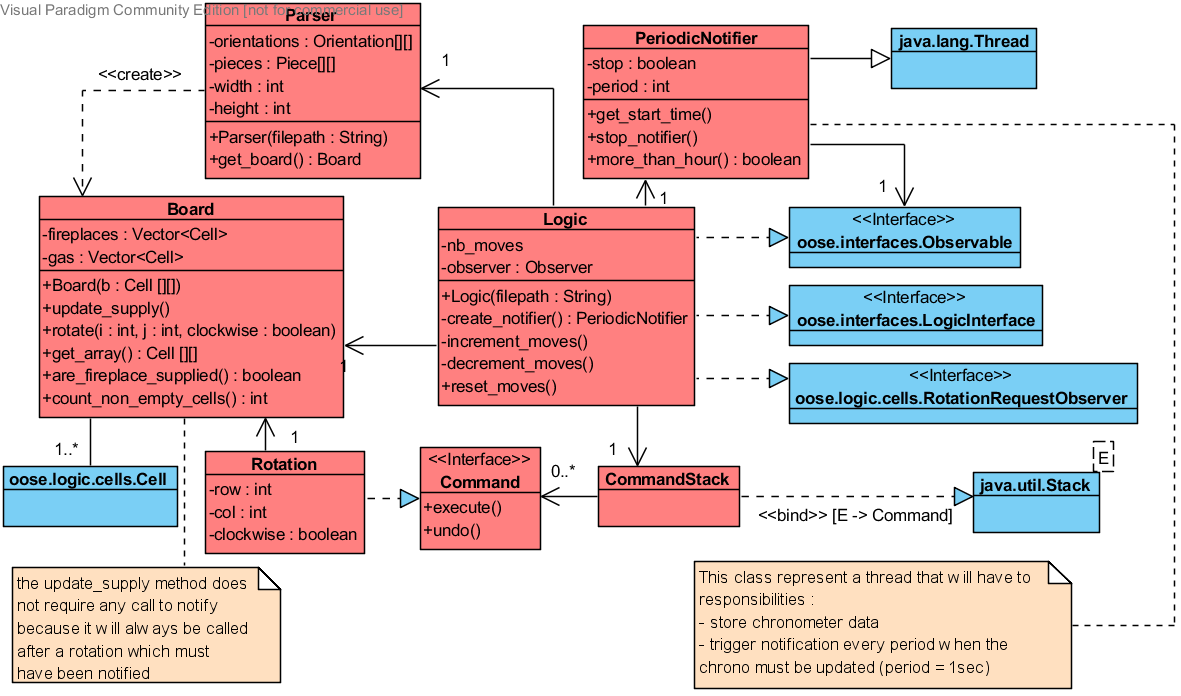
\includegraphics[angle=90,scale=1]{logic.png}
	\caption{Logic core}
	\label{fig:logic}
\end{figure}
\begin{figure}
	\center
	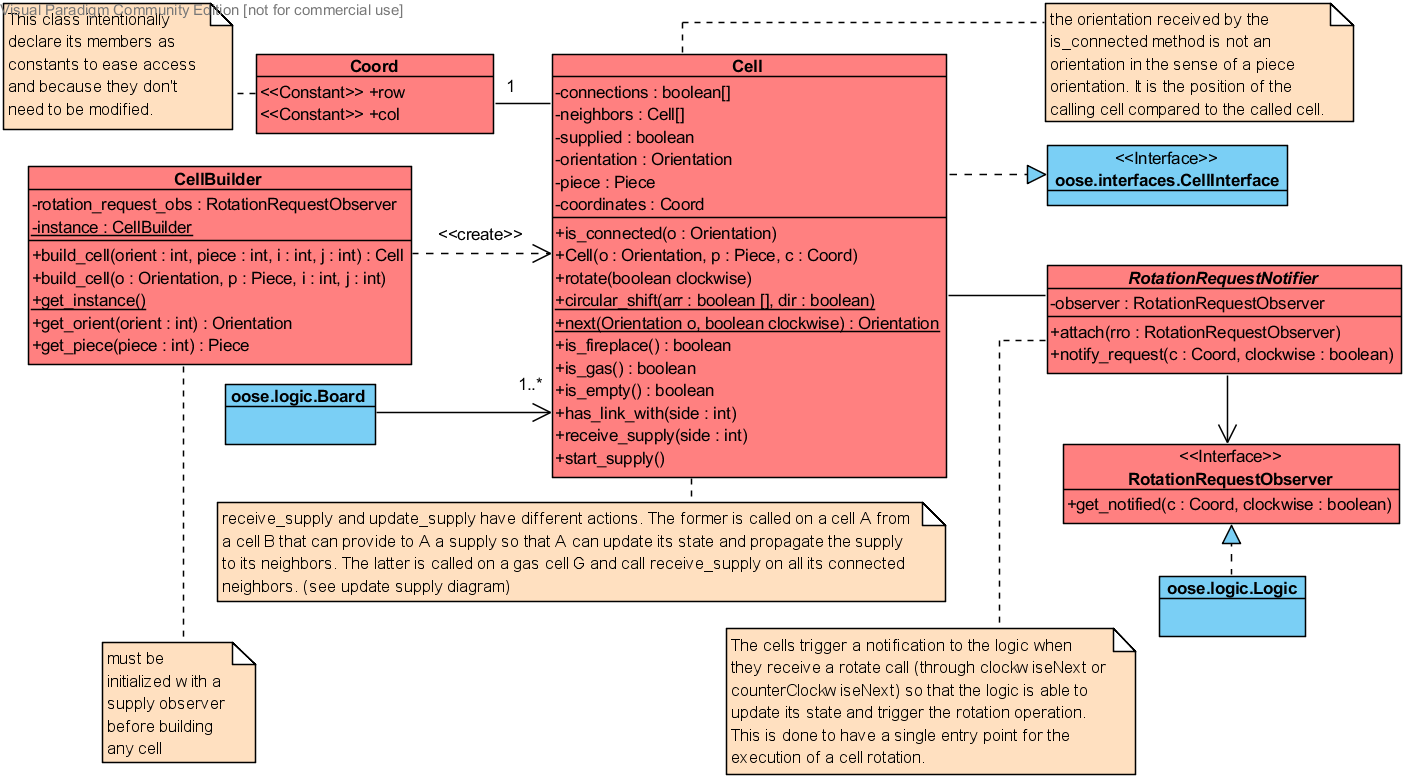
\includegraphics[angle=90,scale=1]{cells.png}
	\caption{Cells}
	\label{fig:cells}
\end{figure}
\subsection{Sequence diagrams}
\begin{figure}
	\center
	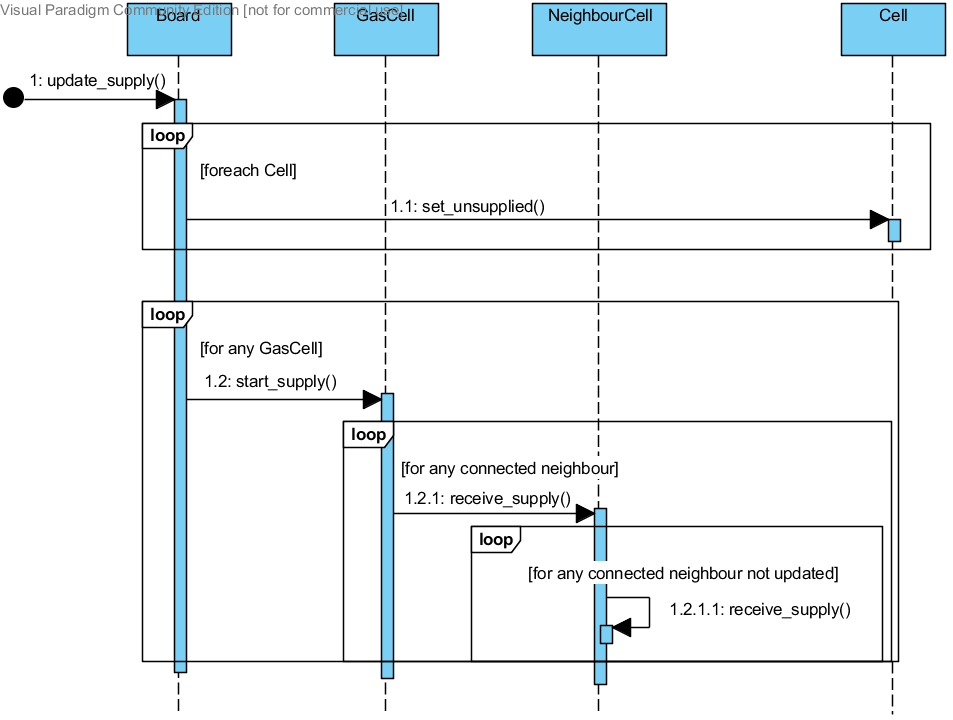
\includegraphics[angle=90,scale=1]{supply_update.png}
	\caption{Supply update}
	\label{fig:sup_update}
\end{figure}
\begin{figure}
	\center
	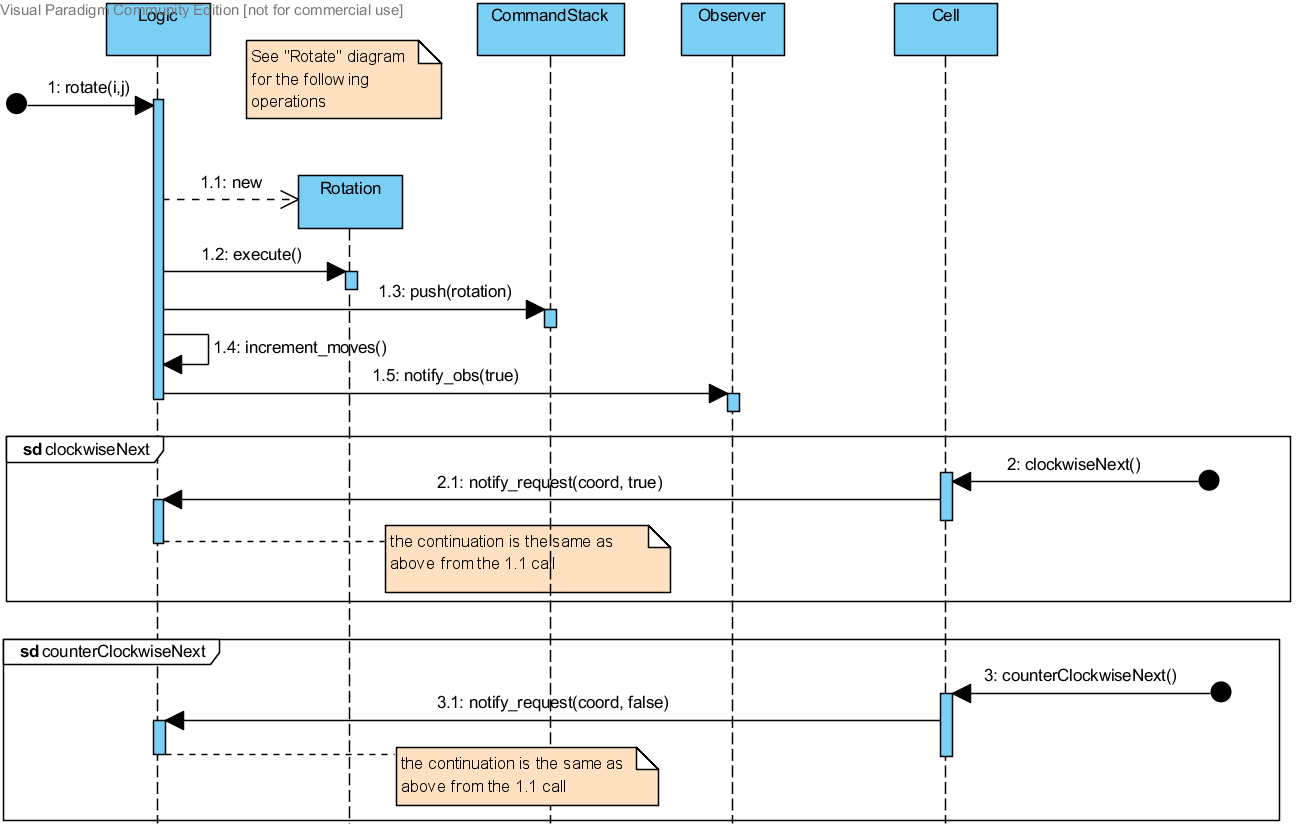
\includegraphics[angle=90,scale=1]{rotation_request.png}
	\caption{Rotation request}
	\label{fig:rot_request}
\end{figure}
\begin{figure}
	\center
	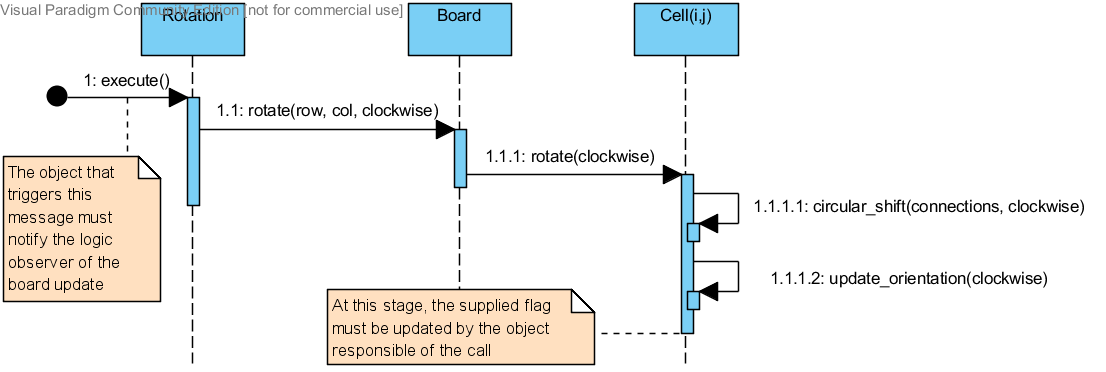
\includegraphics[angle=90,scale=1]{rotation.png}
	\caption{Rotation}
	\label{fig:rotation}
\end{figure}
\begin{figure}
	\center
	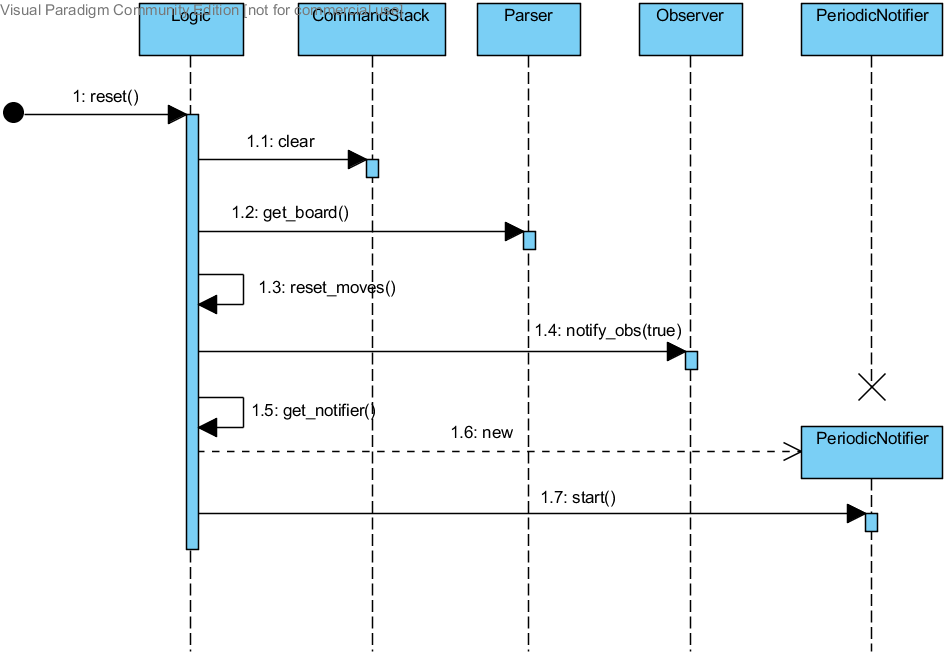
\includegraphics[angle=90,scale=1]{reset.png}
	\caption{Reset}
	\label{fig:reset}
\end{figure}
\begin{figure}
	\center
	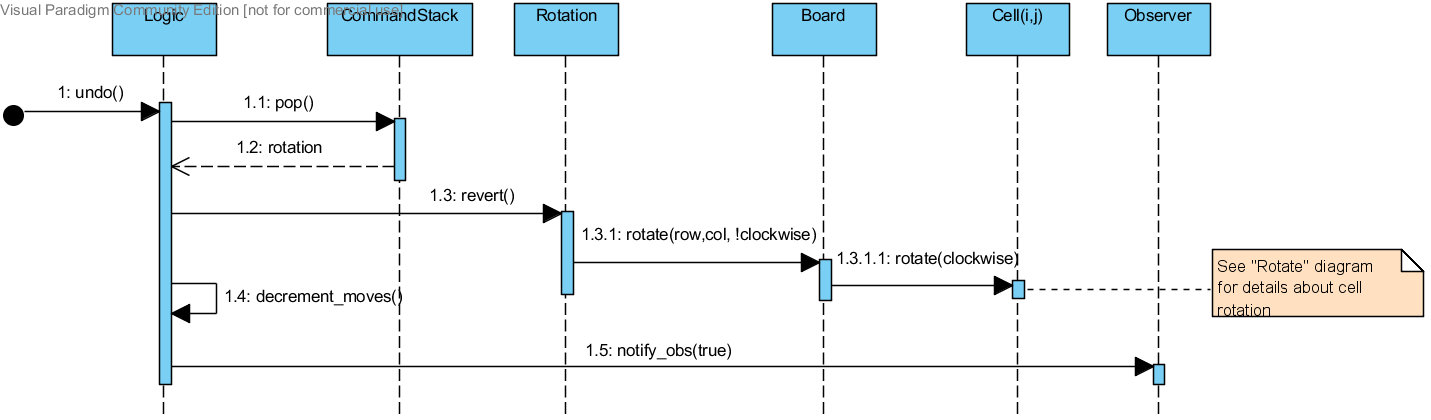
\includegraphics[angle=90,scale=1]{undo.png}
	\caption{Undo}
	\label{fig:undo}
\end{figure}
\end{document}
